\documentclass[10pt]{article}
\def\withcolors{1}
\def\withnotes{1}
\def\withindex{0}
\usepackage[T1]{fontenc}
\usepackage[utf8]{inputenc}

%% Eye-candy
\usepackage{lmodern}
\usepackage{xspace}                                     % Smart spacing with \xspace
\usepackage[protrusion=true,expansion=true]{microtype}  % Improve font rendering

% Striking out text
\usepackage[normalem]{ulem}

%% Math
\usepackage{amsfonts,amsmath,amssymb, amsthm, mathtools}
\usepackage{thm-restate}
\usepackage{dsfont} % For the indicator symbol

% Algorithm environment
\usepackage{algorithmicx,algpseudocode,algorithm}

% Colors (with names)
\usepackage[usenames,dvipsnames,table]{xcolor}

% Quotes: \blockquote command
\usepackage{csquotes}

% Relative sizes for text
\usepackage{relsize}

% Bibliography
%\usepackage[numbers]{natbib}

% Required for the table of results
\usepackage{multirow}
\usepackage{chngpage} % allows for temporary adjustment of side margins

% For the commands such as \capitalisewords
\usepackage{mfirstuc}

% Graphics
\usepackage{tikz}
\usetikzlibrary{arrows}
\usetikzlibrary{calc,decorations.pathmorphing,patterns}

% For indexing
\ifnum\withindex=1
  \usepackage{makeidx}
  \usepackage{ifthen}
  \newcommand\indexed[2][]{\ifthenelse{\equal{#1}{}}{#2\index{#2}}{#2\index{#1}}}
  \makeindex %%%% Enable indexing
\fi
%%\usepackage{showidx} % To debug; does not play well with hyperref

% References and links
\usepackage[backref,colorlinks,citecolor=blue,bookmarks=true,linktocpage]{hyperref}
\usepackage{aliascnt}
\usepackage[numbered]{bookmark}

% Full pages
\usepackage{fullpage}

% Titling
\usepackage{titling}

% Compressed lists
\usepackage[shortlabels]{enumitem}
  \setitemize{noitemsep,topsep=3pt,parsep=2pt,partopsep=2pt} % Uncomment for compact item lists
  \setenumerate{itemsep=1pt,topsep=2pt,parsep=2pt,partopsep=2pt}
  \setdescription{itemsep=1pt}
  
% Package for todo notes.
\ifnum\withnotes=1
  \usepackage[colorinlistoftodos,textsize=scriptsize]{todonotes}
\fi

% Verbatim inputs and code
\usepackage{verbatim}

% Resizable parentheses that work (without the space between \left(#1\right)
\usepackage{mleftright} % \mleft( #1 \mright)

\makeatletter
\@ifundefined{theorem}{%
  % Theorems (each with its own style, all same counter). Cf. http://ftp.math.purdue.edu/mirrors/ctan.org/macros/latex/contrib/hyperref/doc/manual.pdf, p.17
  \theoremstyle{plain} %% Style
  	\newtheorem{theorem}{Theorem}%[section]
  	\newaliascnt{coro}{theorem}
  	  \newtheorem{corollary}[coro]{Corollary}
  	\aliascntresetthe{coro}
  	\newaliascnt{lem}{theorem}
  		\newtheorem{lemma}[lem]{Lemma}
  	\aliascntresetthe{lem}
  	\newaliascnt{clm}{theorem}
  		\newtheorem{claim}[clm]{Claim}
	\aliascntresetthe{clm}
	\newaliascnt{fact}{theorem}
 	 	\newtheorem{fact}[theorem]{Fact}
	\aliascntresetthe{fact}
  	\newtheorem*{unnumberedfact}{Fact}
  \newaliascnt{prop}{theorem}
  		\newtheorem{proposition}[prop]{Proposition}
	\aliascntresetthe{prop}
	\newaliascnt{conj}{theorem}
  		\newtheorem{conjecture}[conj]{Conjecture}
	\aliascntresetthe{conj}
  \theoremstyle{remark} %% Style
  	\newtheorem{remark}[theorem]{Remark}
  	\newtheorem{question}[theorem]{Question}
  	\newtheorem*{notation}{Notation}
 	 \newtheorem{example}[theorem]{Example}
  \theoremstyle{definition} %% Style
  	\newaliascnt{defn}{theorem}
 		 \newtheorem{definition}[defn]{Definition}
 	 \aliascntresetthe{defn}
}{}
\makeatother
\providecommand*{\lemautorefname}{Lemma} % For \autoref{} to know the name of lemmas
\providecommand*{\clmautorefname}{Claim}
\providecommand*{\propautorefname}{Proposition}
\providecommand*{\coroautorefname}{Corollary}
\providecommand*{\defnautorefname}{Definition}
\newenvironment{proofof}[1]{\begin{proof}[Proof of {#1}]}{\end{proof}}

%% \email{} command
\providecommand{\email}[1]{\href{mailto:#1}{\nolinkurl{#1}\xspace}}

%% Remarks and notes
\ifnum\withcolors=1
  \newcommand{\new}[1]{{\color{red} {#1}}} % new
  \newcommand{\newer}[1]{{\color{blue} {#1}}} % even newer
  \newcommand{\newest}[1]{{\color{orange} {#1}}} % even even newer
  \newcommand{\newerest}[1]{{\color{blue!10!black!40!green} {#1}}} % you get the idea.
  \newcommand{\ccolor}[1]{{\color{RubineRed}#1}} % Clement
\else
  \newcommand{\new}[1]{{{#1}}}
  \newcommand{\newer}[1]{{{#1}}}
  \newcommand{\newest}[1]{{{#1}}}
  \newcommand{\newerest}[1]{{{#1}}}
  \newcommand{\ccolor}[1]{{#1}}
\fi

\ifnum\withnotes=1
  \newcommand{\cnote}[1]{\par\ccolor{\textbf{C: }\sf #1}} % Clement
  \newcommand{\todonote}[2][]{\todo[size=\scriptsize,color=red!40,#1]{#2}}  
	\newcommand{\questionnote}[2][]{\todo[size=\scriptsize,color=blue!30]{#2}}
	\newcommand{\todonotedone}[2][]{\todo[size=\scriptsize,color=green!40]{$\checkmark$ #2}}
	\newcommand{\todonoteinline}[2][]{\todo[inline,size=\scriptsize,color=orange!40,#1]{#2}}  
  \newcommand{\marginnote}[1]{\todo[color=white,linecolor=black]{{#1}}}
\else
  \newcommand{\cnote}[1]{}
  \newcommand{\todonote}[2][]{\ignore{#2}}
	\newcommand{\questionnote}[2][]{\ignore{#2}}
	\newcommand{\todonotedone}[2][]{\ignore{#2}}
	\newcommand{\todonoteinline}[2][]{\ignore{#2}}
  \newcommand{\marginnote}[1]{\ignore{#1}}
\fi
\newcommand{\ignore}[1]{\leavevmode\unskip} % eat unnecessary spaces before
\newcommand{\cmargin}[1]{\questionnote{\ccolor{#1}}} % Clement

% Shortcuts
\newcommand{\eps}{\ensuremath{\varepsilon}\xspace}
\newcommand{\Algo}{\ensuremath{\mathcal{A}}\xspace} % Algorithm A
\newcommand{\Tester}{\ensuremath{\mathcal{T}}\xspace} % Testing algorithm T
\newcommand{\Learner}{\ensuremath{\mathcal{L}}\xspace} % Learning algorithm L
\newcommand{\property}{\ensuremath{\mathcal{P}}\xspace} % Property P
\newcommand{\class}{\ensuremath{\mathcal{C}}\xspace} % Class C
\newcommand{\eqdef}{\stackrel{\rm def}{=}}
\newcommand{\eqlaw}{\stackrel{\mathcal{L}}{=}}
\newcommand{\accept}{\textsf{ACCEPT}\xspace}
\newcommand{\fail}{\textsf{FAIL}\xspace}
\newcommand{\reject}{\textsf{REJECT}\xspace}
\newcommand{\opt}{{\textsc{opt}}\xspace}
\newcommand{\half}{\frac{1}{2}}
\newcommand{\domain}{\ensuremath{\Omega}\xspace} % Domain of a distribution (default notation)
\newcommand{\distribs}[1]{\Delta\!\left(#1\right)} % Domain of a distribution (default notation)
\newcommand{\yes}{{\sf{}yes}\xspace}
\newcommand{\no}{{\sf{}no}\xspace}
\newcommand{\dyes}{{\cal Y}}
\newcommand{\dno}{{\cal N}}

% Complexity
\newcommand{\littleO}[1]{{o\mleft( #1 \mright)}}
\newcommand{\bigO}[1]{{O\mleft( #1 \mright)}}
\newcommand{\bigOSmall}[1]{{O\big( #1 \big)}}
\newcommand{\bigTheta}[1]{{\Theta\mleft( #1 \mright)}}
\newcommand{\bigOmega}[1]{{\Omega\mleft( #1 \mright)}}
\newcommand{\bigOmegaSmall}[1]{{\Omega\big( #1 \big)}}
\newcommand{\tildeO}[1]{\tilde{O}\mleft( #1 \mright)}
\newcommand{\tildeTheta}[1]{\operatorname{\tilde{\Theta}}\mleft( #1 \mright)}
\newcommand{\tildeOmega}[1]{\operatorname{\tilde{\Omega}}\mleft( #1 \mright)}
\providecommand{\poly}{\operatorname*{poly}}

% Influence
\newcommand{\totinf}[1][f]{{\mathbf{Inf}[#1]}}
\newcommand{\infl}[2][f]{{\mathbf{Inf}_{#1}(#2)}}
\newcommand{\infldeg}[3][f]{{\mathbf{Inf}_{#1}^{#2}(#3)}}

% Sets and indicators
\newcommand{\setOfSuchThat}[2]{ \left\{\; #1 \;\colon\; #2\; \right\} } 			% sets such as "{ elems | condition }"
\newcommand{\indicSet}[1]{\mathds{1}_{#1}}                                              % indicator function
\newcommand{\indic}[1]{\indicSet{\left\{#1\right\}}}                                             % indicator function
\newcommand{\disjunion}{\amalg}%\coprod, \dotcup...

% Distance
\newcommand{\dtv}{\operatorname{d}_{\rm TV}}
\newcommand{\kl}{\operatorname{KL}}
\newcommand{\dhell}{\operatorname{d_{\rm{}H}}}
\newcommand{\hellinger}[2]{{\dhell\mleft({#1, #2}\mright)}}
\newcommand{\kldiv}[2]{{\kl\mleft({#1 \,\|\, #2}\mright)}}
\newcommand{\kolmogorov}[2]{{\operatorname{d_{\rm{}K}}\mleft({#1, #2}\mright)}}
\newcommand{\totalvardistrestr}[3][]{{\dtv^{#1}\mleft({#2, #3}\mright)}}
\newcommand{\totalvardist}[2]{\totalvardistrestr[]{#1}{#2}}
%\newcommand{\chisquarerestr}[3][]{{\operatorname{d}^{#1}_{\chi^2}\mleft({#2 \mid\mid #3}\mright)}}
\newcommand{\chisquare}[2]{{\chi^2\mleft({#1 \mid\mid #2}\mright)}}
\newcommand{\dist}[2]{\operatorname{dist}\mleft({#1, #2}\mright)}

% Restriction (functions, sequences, etc.)
\newcommand\restr[2]{{% we make the whole thing an ordinary symbol
  \left.\kern-\nulldelimiterspace % automatically resize the bar with \right
  #1 % the function
  \vphantom{\big|} % pretend it's a little taller at normal size
  \right|_{#2} % this is the delimiter
  }}

% Probability
\newcommand{\proba}{\Pr}
\newcommand{\probaOf}[1]{\proba\!\left[\, #1\, \right]}
\newcommand{\probaCond}[2]{\proba\!\left[\, #1 \;\middle\vert\; #2\, \right]}
\newcommand{\probaDistrOf}[2]{\proba_{#1}\left[\, #2\, \right]}

% Support of a distribution/function
\newcommand{\supp}[1]{\operatorname{supp}\!\left(#1\right)}

% Expectation & variance
\newcommand{\expect}[1]{\mathbb{E}\!\left[#1\right]}
\newcommand{\expectCond}[2]{\mathbb{E}\!\left[\, #1 \;\middle\vert\; #2\, \right]}
\newcommand{\shortexpect}{\mathbb{E}}
\newcommand{\var}{\operatorname{Var}}

% Distributions
\newcommand{\uniform}{\ensuremath{\mathcal{U}}}
\newcommand{\uniformOn}[1]{\ensuremath{\uniform\!\left( #1 \right) }}
\newcommand{\geom}[1]{\ensuremath{\operatorname{Geom}\!\left( #1 \right)}}
\newcommand{\bernoulli}[1]{\ensuremath{\operatorname{Bern}\!\left( #1 \right)}}
\newcommand{\bern}[2]{\ensuremath{\operatorname{Bern}^{#1}\!\left( #2 \right)}}
\newcommand{\binomial}[2]{\ensuremath{\operatorname{Bin}\!\left( #1, #2 \right)}}
\newcommand{\poisson}[1]{\ensuremath{\operatorname{Poisson}\!\left( #1 \right) }}
\newcommand{\gaussian}[2]{\ensuremath{ \mathcal{N}\!\left(#1,#2\right) }}
\newcommand{\gaussianpdf}[2]{\ensuremath{ g_{#1,#2}}}
\newcommand{\betadistr}[2]{\ensuremath{ \operatorname{Beta}\!\left( #1, #2 \right) }}

% Norms
\newcommand{\norm}[1]{\lVert#1{\rVert}}
\newcommand{\normone}[1]{{\norm{#1}}_1}
\newcommand{\normtwo}[1]{{\norm{#1}}_2}
\newcommand{\norminf}[1]{{\norm{#1}}_\infty}
\newcommand{\abs}[1]{\left\lvert #1 \right\rvert}
\newcommand{\dabs}[1]{\lvert #1 \rvert}
\newcommand{\dotprod}[2]{ \left\langle #1,\xspace #2 \right\rangle } 			% <a,b>
\newcommand{\ip}[2]{\dotprod{#1}{#2}} 			% shortcut

\newcommand{\vect}[1]{\mathbf{#1}} 			% shortcut

% Ceiling and floor
\newcommand{\clg}[1]{\left\lceil #1 \right\rceil}
\newcommand{\flr}[1]{\left\lfloor #1 \right\rfloor}

% Common sets
\newcommand{\R}{\ensuremath{\mathbb{R}}\xspace}
\newcommand{\C}{\ensuremath{\mathbb{C}}\xspace}
\newcommand{\Q}{\ensuremath{\mathbb{Q}}\xspace}
\newcommand{\Z}{\ensuremath{\mathbb{Z}}\xspace}
\newcommand{\N}{\ensuremath{\mathbb{N}}\xspace}
\newcommand{\cont}[1]{\ensuremath{\mathcal{C}^{#1}}}

% Oracles and variants
\newcommand{\ICOND}{{\sf INTCOND}\xspace}
\newcommand{\EVAL}{{\sf EVAL}\xspace}
\newcommand{\CDFEVAL}{{\sf CEVAL}\xspace}
\newcommand{\STAT}{{\sf STAT}\xspace}
\newcommand{\SAMP}{{\sf SAMP}\xspace}
\newcommand{\COND}{{\sf COND}\xspace}
\newcommand{\PCOND}{{\sf PAIRCOND}\xspace}
\newcommand{\ORACLE}{{\sf ORACLE}\xspace}

%% Terminology
\newcommand{\pdfsamp}{dual\xspace}
\newcommand{\cdfsamp}{cumulative dual\xspace}
\newcommand{\Pdfsamp}{\expandafter\capitalisewords\expandafter{\pdfsamp}}
\newcommand{\Cdfsamp}{\expandafter\capitalisewords\expandafter{\cdfsamp}}

% L_p norms
\newcommand{\lp}[1][1]{\ell_{#1}}

% Convolution
\DeclareMathOperator{\convolution}{\ast}

%% Terminology
\newcommand{\D}{\ensuremath{D}}
\newcommand{\distrD}{\ensuremath{\mathcal{D}}}
\newcommand{\birge}[2][\D]{\Phi_{#2}(#1)}
\newcommand{\iid}{i.i.d.\xspace}

% Sign
\DeclareMathOperator{\sign}{sgn}

%% Roman numerals
\makeatletter
\newcommand{\rom}[1]{\romannumeral #1}
\newcommand{\Rom}[1]{\expandafter\@slowromancap\romannumeral #1@}
\newcommand{\century}[2][th]{\Rom{#2}\textsuperscript{#1}}
\makeatother

% Hyperref and \autoref{} -- names
\renewcommand{\sectionautorefname}{Section} % To have "Section 5" instead of "section 5" with \autoref{}
\renewcommand{\chapterautorefname}{Chapter} % To have "Chapter 5" instead of "chapter 5" with \autoref{}
\renewcommand{\subsectionautorefname}{Section} % To have "Section 5" instead of "subsection 5" with \autoref{}
\renewcommand{\subsubsectionautorefname}{Section} % To have "Section 5" instead of "subsubsection 5" with \autoref{}
\def\algorithmautorefname{Algorithm}


%%%%%%%%%%%%%%%%%%%%%%%%%%%%%%%%%%%%%%%%%%%%%%%%%%%%%%%%%%%%%%%%%
% Add author and title info to PDF (and handles multiple authors)
%%%%%%%%%%%%%%%%%%%%%%%%%%%%%%%%%%%%%%%%%%%%%%%%%%%%%%%%%%%%%%%%%
\makeatletter
  \AtBeginDocument{
  \begingroup
  \toks@={}%
  \toksdef\toks@@=2 %
  \toks@@={}%
  \long\def\@ReturnFiFi#1#2\fi\fi{\fi\fi#1}%
  \def\scan@author#1#2 \and#3\@nil{%
  \ifx\\#3\\%
    \ifcase#1 %
      \toks@={#2}%
    \else
      \ifnum#1>1 %
        \toks@=\expandafter{%
          \the\expandafter\toks@\expandafter,\expandafter\space
          \the\toks@@
        }%
      \fi
      \toks@=\expandafter{\the\toks@\space and #2}%
    \fi
    \else
      \ifcase#1 %
        \toks@={#2}%
        \@ReturnFiFi{%
          \scan@author1#3\@nil
        }%
      \else
        \ifnum#1>1 %
          \toks@=\expandafter{%
            \the\expandafter\toks@\expandafter,\expandafter\space
            \the\toks@@
          }%
      \fi
      \toks@@={#2}%
      \@ReturnFiFi{%
        \scan@author2#3\@nil
      }%
    \fi
  \fi
  }%
  \expandafter\expandafter\expandafter\scan@author
  \expandafter\expandafter\expandafter0%
  \expandafter\@author\space\and\@nil
  \edef\x{\endgroup
  \noexpand\hypersetup{pdfauthor={\the\toks@}}%
  }%
  \x
  }
\makeatother


\newcommand{\dst}{\varepsilon}
\newcommand{\ab}{k}
\newcommand{\ns}{n}
\newcommand{\dims}{d}

\newcommand{\p}{\mathbf{p}}
\newcommand{\q}{\mathbf{q}}

\renewcommand{\eqdef}{\coloneqq}
\theoremstyle{plain}
\newtheorem{problem}[theorem]{Problem}

\usepackage{filecontents}

\title{Testing Gaussians, in many ways}
\date{September, 2020}

\begin{document}
\begin{flushleft}\sf\footnotesize
\makeatletter
\@date~- \today \hfill \@title
\makeatother
\end{flushleft}
\vspace{5mm}

The goal of this short note is to record tight bounds on various testing problems for $\dims$-dimensional Gaussians. Let $\q$ denote the standard Gaussian, i.e., $\q\eqdef \gaussian{\mathbf{0}}{I_\dims}$. Any mistake or imprecision is mine.
\begin{problem}[TV Testing Under Identity Covariance Assumption]
  \label{problem:tv:identitycov}
  Given $\dst \in(0,1]$ and i.i.d.\ samples from some $\p\eqdef\gaussian{\mu}{I_\dims}$ with unknown $\mu$, distinguish between $\p = \q$ and $\totalvardist{\p}{\q }> \dst$.
\end{problem}
\hfill \textbf{Sample complexity:} $\bigTheta{\sqrt{\dims}/\dst^2}$. 

\begin{problem}[Mean Norm Estimation Under Identity Covariance Assumption]
  \label{problem:mean:identitycov}
  Given $\dst \in(0,1]$ and i.i.d.\ samples from some $\p\eqdef\gaussian{\mu}{I_\dims}$ with unknown $\mu$, learn $\normtwo{\mu}$ to an additive $\dst$.
\end{problem}
\hfill \textbf{Sample complexity:} $\bigTheta{\sqrt{\dims}/\dst^2}$. 

\begin{problem}[Mean Estimation Under Identity Covariance Assumption (a.k.a.\ Gaussian Location Model)]
  \label{problem:mean:identitycov:learn}
  Given $\dst \in(0,1]$ and i.i.d.\ samples from some $\p\eqdef\gaussian{\mu}{I_\dims}$ with unknown $\mu$, learn $\mu$ to $\lp[2]$ norm $\dst$.
\end{problem}
\hfill \textbf{Sample complexity:} $\bigTheta{\dims/\dst^2}$. 

\begin{problem}[TV Testing]
  \label{problem:tv:general}
  Given $\dst \in(0,1]$ and i.i.d.\ samples from some $\p\eqdef\gaussian{\mu}{\Sigma}$ with unknown $\mu,\Sigma$, distinguish between $\p = \q$ and $\totalvardist{\p}{\q }> \dst$.
\end{problem}
\hfill \textbf{Sample complexity:} $\bigTheta{\dims/\dst^2}$. 

\begin{problem}[Mean Testing]
  \label{problem:mean:testing:standard}
  Given $\dst \in(0,1]$ and i.i.d.\ samples from some $\p\eqdef\gaussian{\mu}{\Sigma}$ with unknown $\mu,\Sigma$, distinguish between $\p = \q$ and $\normtwo{\mu} > \dst$.
\end{problem}
\hfill \textbf{Sample complexity:} $\bigTheta{\sqrt{\dims}/\dst^2}$. 

\begin{problem}[Covariance Norm Estimation, Operator Norm]
  \label{problem:cov:learn:norm:op}
  Given $\dst \in(0,1], \kappa >0$ and i.i.d.\ samples from some $\p\eqdef\gaussian{\mu}{\Sigma}$ with unknown $\mu,\Sigma$ such that $\norm{\Sigma- I_\dims}_{\rm op}\leq \kappa$, learn $\norm{\Sigma - I_\dims}_{\rm op}$ to an additive $\dst$.
\end{problem}
\hfill \textbf{Sample complexity:} $\bigTheta{\kappa^2\dims/\dst^2}$. 

\begin{problem}[Covariance Estimation, Operator Norm]
  \label{problem:cov:learn:op}
  Given $\dst \in(0,1], \kappa >0$ and i.i.d.\ samples from some $\p\eqdef\gaussian{\mu}{\Sigma}$ with unknown $\mu,\Sigma$ such that $\norm{\Sigma- I_\dims}_{\rm op}\leq \kappa$, learn $\Sigma$ to $\norm{\cdot}_{\rm op}$ norm $\dst$.
\end{problem}
\hfill \textbf{Sample complexity:} $\bigTheta{\kappa^2\dims/\dst^2}$. 

\begin{problem}[Covariance Norm Estimation, Frobenius Norm]
  \label{problem:cov:learn:norm:frob}
  Given $\dst \in(0,1], \kappa >0$ and i.i.d.\ samples from some $\p\eqdef\gaussian{\mu}{\Sigma}$ with unknown $\mu,\Sigma$ such that $\norm{\Sigma- I_\dims}_{F}\leq \kappa$, learn $\norm{\Sigma-I_\dims}_{F}$ to an additive $\dst$.
\end{problem}
\hfill \textbf{Sample complexity:} $\bigTheta{\kappa^2\dims/\dst^2}$. 

\begin{problem}[Covariance Estimation, Frobenius Norm]
  \label{problem:cov:learn:frob}
  Given $\dst \in(0,1], \kappa>0$ and i.i.d.\ samples from some $\p\eqdef\gaussian{\mu}{\Sigma}$ with unknown $\mu,\Sigma$ such that $\norm{\Sigma - I_\dims}_{F}\leq \kappa$, learn $\Sigma$ to $\norm{\cdot}_{F}$ norm $\dst$.
\end{problem}
\hfill \textbf{Sample complexity:} $\bigTheta{\kappa^2\dims^2/\dst^2}$. 

Finally, this one will be rather useful to prove lower bounds, as we will see later, but also makes sense by itself~--~who has never wanted to test whether the vector of eigenvalues of a covariance matrix had large $\lp[2]$ norm?
\begin{problem}[Covariance Norm Testing, Frobenius Norm]
  \label{problem:cov:test:norm:frob}
  Given $\dst \in(0,1]$ and i.i.d.\ samples from some $\p\eqdef\gaussian{\mathbf{0}}{\Sigma}$ with unknown $\Sigma$, distinguish between $\p=\q$ and $\norm{\Sigma-I_\dims}_{F}>\dst$.
\end{problem}
\hfill \textbf{Sample complexity:} $\bigTheta{\dims/\dst^2}$. 

%%%%%%%%%%%%%%%%%%%%%%%%%%%%%%%%%%%%%%%%
\section{A crucial fact}
The starting point of many of those results will be that the total variation distance between two high-dimensional Gaussians~--~and thus, a fortiori, the distance to the standard one, $\q$~-- is characterized by the appropriate distances between their parameters:
\begin{fact}
  \label{fact:tv:parameters}
  Let $\p\eqdef\gaussian{\mu}{\Sigma}$. Then
  $
      \totalvardist{\p}{\q} \leq 2\max\mleft(  \normtwo{\mu}, \norm{\Sigma-I_\dims}_F \mright)\,.
  $
  Conversely, we have $\totalvardist{\p}{\q} \geq C\min(1,\max\mleft(  \normtwo{\mu}, \norm{\Sigma-I_\dims}_F \mright))$, for some absolute constant $C>0$.
\end{fact}
\begin{proof}
There are many references for this, with various degrees of complexity and tightness of the constants; see, e.g.,~\cite[Corollary~1.4.6]{Li2018}, or~\cite[Theorem~1.3]{DevroyeMR2018}. We here give a self-contained proof of the upper bound.\footnote{But would be delighted to be pointed to a simple proof of the general statement, as we do not particularly care about obtaining the tightest constants possible.}
We start by the (exact) expression of the Kullback--Leibler divergence between $\p$ and $\q$. Denoting the $\dims$ eigenvalues of $\Sigma$ by $0\leq \lambda_1\leq \dots\leq \lambda_\dims$, we have, using the ``folklore'' expression for the divergence between two arbitrary multivariate Gaussians,\footnote{Folklore, in that case, is synonymous with Wikipedia~\cite{wiki:KL}.}
\[
  \kldiv{\p}{\q} 
  = \frac{1}{2}\mleft(  \normtwo{\mu}^2 + \operatorname{Tr}\Sigma -\dims - \log \det \Sigma \mright)
  = \frac{1}{2}\mleft(  \normtwo{\mu}^2 + \sum_{i=1}^\dims (\lambda_i - 1 - \log \lambda_i) \mright)
\]
Assume for now (we will argue later why it is safe to do so) that $\abs{\lambda_i - 1}\leq 1/2$ for all $i$. In that case, since the very convenient inequality\footnote{Which is inspired by looking at the Taylor expansion of $\log$ around $1$: $\log x = (x-1) - \frac{1}{2}(x-1)^2 + o((x-1)^2)$.}
$
  x-1 \leq \log x + (x-1)^2
$ holds for all $x\geq 1/2$, and 
we get 
\[
  \kldiv{\p}{\q} \leq  \frac{1}{2}\mleft(  \normtwo{\mu}^2 + \sum_{i=1}^\dims (\lambda_i - 1)^2 \mright) = \frac{1}{2}\mleft(  \normtwo{\mu}^2 + \norm{\Sigma-I_\dims}_F^2 \mright)
  \leq \max\mleft(  \normtwo{\mu}^2, \norm{\Sigma-I_\dims}_F^2 \mright)\,,
\]
where we used that, for positive semi-definite matrices the Frobenius norm is the $\lp[2]$ norm of the vector of eigenvalues. Now, by Pinsker's inequality, we get
\[
    \totalvardist{\p}{\q} \leq \sqrt{\frac{1}{2}\kldiv{\p}{\q}} \leq \frac{1}{\sqrt{2}}\max\mleft(  \normtwo{\mu}, \norm{\Sigma-I_\dims}_F \mright)
\]
which gives the claim. Almost: it remains to explain why we could assume that $\abs{\lambda_i - 1}\leq 1/2$ for all $i$. This is just because, otherwise, we have
$\norm{\Sigma-I_\dims}_F \geq \max_{1\leq i \leq \dims} \abs{\lambda_i - 1} > 1/2$, and since the total variation distance is always at most one we have $\totalvardist{\p}{\q} < 2\norm{\Sigma-I_\dims}_F$, and the claim holds as well.

%%%%%%%%%%%%%%%%%%%%%%%%%%
%% Bonus useless stuff! %%
%%%%%%%%%%%%%%%%%%%%%%%%%%
% To see that, suppose without loss of generality that $\abs{\lambda_1 - 1} > 1/2$, let $v$ be the eigenvector associated with $\lambda_1$. Let $\p'$ be the (Gaussian) distribution of $\dotprod{X}{v}$ when $X\sim\p$, and $\q'$ the same thing for $\q$: note that $\p'=\gaussian{0}{1}$ and $\q'=\gaussian{\dotprod{\mu}{v}}{\lambda_1}$. We then have
% \[
%     \totalvardist{\p}{\q} \geq \totalvardist{\p'}{\q'} \geq \frac{1}{2}\totalvardist{\p'^{\otimes 2}}{\q'^{\otimes 2}} = \frac{1}{2}\totalvardist{\gaussian{0}{\lambda_1}}{\gaussian{0}{1}}
% \]
% where the first inequality is the data processing inequality (DPI), the second is subadditivity of total variation distance,\footnote{That is, in general, $\totalvardist{\p_1\otimes\p_2}{\q_1\otimes\q_2} \leq \totalvardist{\p_1}{\q_1}+\totalvardist{\p_2}{\q_2}$, as a consequence of the triangle inequality.} and the third is again the DPI by using the transformation $f(x,y)=\frac{x-y}{\sqrt{2}}$ and noting that the distribution of $f(X,Y)$ for $(X,Y)\sim\p'^{\otimes 2}$ (resp., $(X,Y)\sim\q'^{\otimes 2}$) is exactly $\gaussian{0}{\lambda_1}$ (resp., $\gaussian{0}{1}$). Why did we do all this? Because now, lower bounding $\totalvardist{\gaussian{0}{\lambda_1}}{\gaussian{0}{1}}$ is (relatively) easy: by lower bounding the integral defining the total variation distance, one can check that this is at least some absolute constant; specifically,
% \[
% \totalvardist{\gaussian{0}{\lambda_1}}{\gaussian{0}{1}} \geq \min\mleft(\totalvardist{\gaussian{0}{1/2}}{\gaussian{0}{1}},\totalvardist{\gaussian{0}{3/2}}{\gaussian{0}{1}}\mright) \geq 0.387\,.
% \]
\end{proof}
\emph{Why} do we care about this? This will help us find relations between the problems considered, of the type ``if I have an algorithm for problem $A$, then I can use it to solve problem $B$ with the same sample complexity''~--~in turn allowing us to only prove a few bounds and get the whole picture. 

%%%%%%%%%%%%%%%%%%%%%%%%%%%%%%%%%%%%%%%%
\section{Relationship between problems}
For instance, suppose that we are under the identity-covariance assumption, i.e., promised that $\Sigma=I_\dims$ for the unknown Gaussian $\p$. Then $\p=\q$ is equivalent to $\mu=\mathbf{0}$, and by~\autoref{fact:tv:parameters} we now know that $\totalvardist{\p}{\q}>\dst$ implies $\normtwo{\mu}>\dst/2$. So we have the following (where $A \preceq B$ means ``$A$ requires at most as many samples as $B$''):
\[
      \text{\autoref{problem:tv:identitycov}} \preceq \text{\autoref{problem:mean:identitycov}} \preceq \text{\autoref{problem:mean:identitycov:learn}}
\]
We also have the other following relations:
\[
      \text{\autoref{problem:tv:identitycov}} \preceq \text{\autoref{problem:tv:general}}
\]
(as an algorithm for the more general problem~\autoref{problem:tv:general} can be used for the more specific~\autoref{problem:tv:identitycov}); as well as
\[
      \text{\autoref{problem:tv:identitycov}} \preceq \text{\autoref{problem:mean:testing:standard}}
\]
(because again of~\autoref{fact:tv:parameters}; can you see why?). Finally, we also have
\[
    \text{\autoref{problem:cov:learn:norm:op}} \preceq \text{\autoref{problem:cov:learn:op}}, \qquad \text{\autoref{problem:cov:test:norm:frob}} \preceq \text{\autoref{problem:cov:learn:norm:frob}} \preceq \text{\autoref{problem:cov:learn:frob}}
\]
(again, check you see why~--~the idea is that learning the parameter implies learning its norm which implies testing its magnitude), and
\[
    \text{\autoref{problem:cov:learn:norm:op}} \preceq \text{\autoref{problem:cov:learn:norm:frob}}, \qquad \text{\autoref{problem:cov:learn:op}} \preceq \text{\autoref{problem:cov:learn:frob}}
\]
this time because $\norm{\cdot}_{\rm op}\leq \norm{\cdot}_{F}$. See~\autoref{fig:relations} for a colorful illustration.

\begin{figure}\centering
  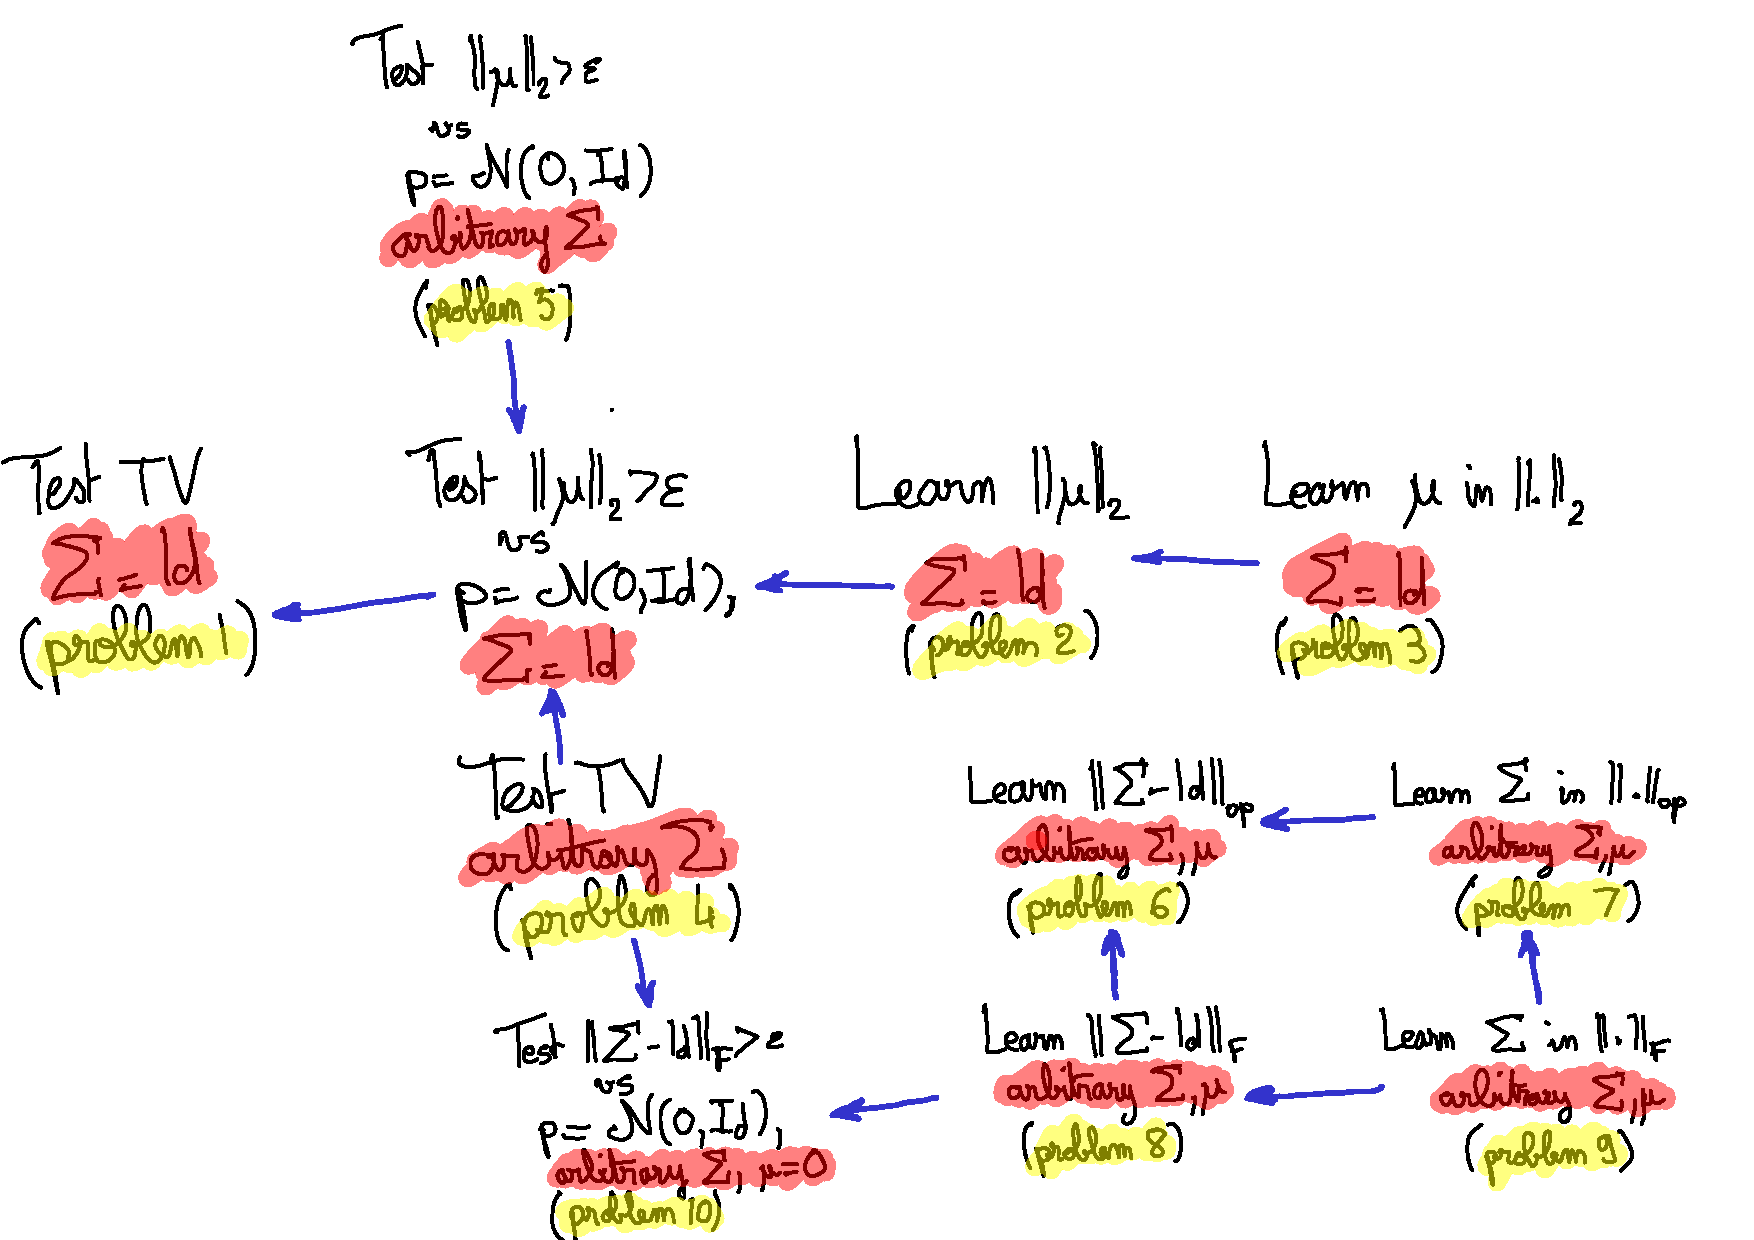
\includegraphics[width=.95\textwidth]{testing-gaussian-fig}
  \caption{\label{fig:relations}Relationships between the different problems considered here (and one extra, in the middle)}
\end{figure}

\begin{remark}
  There is also some relation between~\autoref{problem:tv:general} and the combination (\autoref{problem:mean:testing:standard}+~\autoref{problem:cov:test:norm:frob}), but it is less obvious and a bit more cumbersome. The idea is that (barring quite a few details) if one can solve both~\autoref{problem:mean:testing:standard} and~\autoref{problem:cov:test:norm:frob}, one can solve~\autoref{problem:tv:general} as follows:
  \begin{enumerate}
    \item use the algorithm for~\autoref{problem:mean:testing:standard} to detect if $\normtwo{\mu}\gtrsim \dst$ (and ``reject'' if it is the case)
    \item use the algorithm for~\autoref{problem:cov:test:norm:frob} to detect if $\norm{\Sigma-I_\dims}_F\gtrsim \dst$ (and ``reject'' if it is the case), \emph{but} on new samples of the form $X'\eqdef \frac{X-Y}{\sqrt{2}}$, where $X,Y\sim\p$. This transformation increases the number of samples needed by a factor $2$, but as a result the distribution of those new samples is $\gaussian{\mathbf{0}}{\Sigma}$ (the mean $\mu$ cancels out, the covariance is preserved).
    \item if both tests pass, declare $\p=\q$.
  \end{enumerate}
  Overall, this allows us to distinguish between $\p=\q$ and $\max(\normtwo{\mu},\norm{\Sigma-I_\dims}_F) \ll \dst$, which by~\autoref{fact:tv:parameters} is enough to solve~\autoref{problem:tv:general}.
\end{remark}

%%%%%%%%%%%%%%%%%%%%%%%%%%%%%%%%%%%%%%%%
\section{The proofs, and where to find them}
Given all the relations between problems outlined in the previous section, we don't have as many upper bound lower bounds to prove as one would fear: at least, much fewer that 10 upper and 10 lower bounds.

\begin{itemize}
  \item 
The $\bigOmega{\sqrt{\dims}/\dst^2}$ lower bound for~\autoref{problem:tv:identitycov} is considered folklore, and can be shown, e.g., by Le Cam's two-point method, considering the $2^\dims$ distributions 
\[
    \p_z \eqdef \gaussian{\frac{2\dst}{\sqrt{\dims}}z}{I_\dims}, z\in\{-1,1\}^\dims\,.
\]
Each such $\p_z$ has mean with $\lp[2]$ norm exactly $2\dst$, so an algorithm for~\autoref{problem:tv:identitycov} should allow us to distinguish them from the standard Gaussian $\q$. Even more, if $\ns$ samples are enough for the task, it should allow us to distinguish between the mixture $\frac{1}{2^\dims} \sum_{z\in\{-1,1\}^\dims} \p_z^{\otimes \ns}$ (pick one $\p_z$ uniformly at random, draw $\ns$ samples from it) and $\gaussian{\mathbf{0}}{I_{\dims}}^{\otimes \ns}$ ($\ns$ samples from the standard Gaussian). This in turn can be shown to require $\ns=\bigOmega{\sqrt{\dims}/\dst^2}$ samples (see, for instance,~\cite[Chapter~23]{Wu17}).
  \item
The $\bigO{\sqrt{\dims}/\dst^2}$ upper bound for~\autoref{problem:mean:identitycov} is also ``folklore,''\footnote{Meaning it is awfully hard to track down a published reference for it, as nobody appears to know any but will swear there must be dozens.} but is achieved by the empirical estimator (considering the squared $\lp[2]$ norm of the empirical estimator, that is, $\normtwo{\frac{1}{\ns}\sum_{i=1}^\ns X^{(j)}}^2$, and doing an expectation+variance+Chebyshev analysis). The analysis is not horrendous, although my preference is to divide the $\ns$ samples in two sets $(X^{(j)})_{j=1}^{\ns/2}$ and $(Y^{(j)})_{j=1}^{\ns/2}$ and to use the estimator $\frac{2}{\ns}\sum_{i=1}^{\ns/2} \dotprod{X^{(j)}}{Y^{(j)}}$. I find the computations cleaner.
  \item
The $\bigO{\sqrt{\dims}/\dst^2}$ upper bound for~\autoref{problem:mean:testing:standard} is, oddly, very recent, and can be found in~\cite[Section~4]{CanonneCKLW19}. I find that proof rather suprising and cute.
  \item
The $\bigTheta{\dims/\dst^2}$ upper and lower bound for~\autoref{problem:mean:identitycov:learn} (a question also known as Gaussian Location Model, or GLM) have many proofs, but I strongly recommend~\cite[Section~9.1]{Wu17}, which provides a more general statement and establishes it in an incredibly elegant way.

  \item
The $\bigO{\dims/\dst^2}$ upper and lower bound for~\autoref{problem:mean:identitycov:learn} (a question also known as Gaussian Location Model, or GLM) have many proofs, but I strongly recommend~\cite[Section~9.1]{Wu17}, which provides a more general statement and establishes it in an incredibly elegant way.

  \item
The $\bigOmega{\dims/\dst^2}$ lower bounds for~\autoref{problem:cov:learn:norm:op} and~\autoref{problem:cov:test:norm:frob} both follow from the difficult to distinguish between an identity-covariance matrix and one perturbed by a scaled rank-one matrix, i.e., of the form $I_\dims+\eta vv^\top$. Note that this is a testing (distinguishing) problem for the operator norm, so that implies the same lower bound for~\autoref{problem:cov:learn:norm:op} (estimating that norm) and~\autoref{problem:cov:test:norm:frob} (testing in Frobenius, but Frobenius upper bounds operator norm). This lower bound, proven via Le Cam's two-point method combined with Ingster's method,\footnote{A fancy way to state we upper bound $\chi^2$ distances in a clever (and very useful to know) fashion.} can be found, e.g., in~\cite[Section~24.2]{Wu17}.\footnote{Really, Yihong Wu's lecture notes are a treasure trove.}
  \item
The $\bigO{\dims/\dst^2}$ upper bound for~\autoref{problem:cov:learn:op} can also be found in~\cite[Section~24.2]{Wu17}, and is achieved by the ``obvious'' estimator: the empirical covariance matrix $\widehat{\Sigma}\eqdef \frac{1}{\ns}\sum_{j=1}^\ns X^{(j)}{X^{(j)}}^\top$. A more detailed reference (and a very good one!) for that upper bound is~\cite[Chapter~4.7]{Vershynin18}.
  \item
The $\bigO{\dims/\dst^2}$ and $\bigO{\kappa^2\dims/\dst^2}$ upper bounds for~\autoref{problem:cov:test:norm:frob} and~\autoref{problem:cov:learn:norm:frob} can be found or follow from~\cite{CaiM13}; they are achieved by a unbiased statistic for $\norm{\Sigma-I_\dims}_F^2 = \operatorname{Tr}\mleft((\Sigma-I_\dims)^2\mright)$.
  \item
  All that remains are the $\bigO{\dims^2/\dst^2}$ upper and lower bounds for~\autoref{problem:cov:learn:frob}. I am not sure which reference is best, but~\cite[Section~4.2.2]{DiakonikolasKKLMS16}, or~\cite[Corollary~2.1.12]{Li2018} both show that the upper bound is achieving (again) by the empirical covariance $\widehat{\Sigma}\eqdef \frac{1}{\ns}\sum_{j=1}^\ns X^{(j)}{X^{(j)}}^\top$. I am still tracking down a self-contained reference for the lower bound.
\end{itemize}

%%%%%%%%%% Bibliography
\begin{filecontents}{referencestesting-gaussian.bib}
@misc{ wiki:KL,
    author = "{Wikipedia contributors}",
    title = "Kullback–Leibler divergence --- {Wikipedia}{,} The Free Encyclopedia",
    year = "2020",
    howpublished = "\url{https://en.wikipedia.org/w/index.php?title=Kullback%E2%80%93Leibler_divergence&oldid=983534042}",
    note = "[Online; accessed 15-October-2020]"
  }
  
@phdthesis{Li2018,
  author    = {Jerry Zheng Li},
  title     = {Principled approaches to robust machine learning and beyond},
  school    = {Massachusetts Institute of Technology, Cambridge, {USA}},
  year      = {2018}
}

@misc{Wu17,
  title={Lecture notes for {ECE598YW}: Information-theoretic methods for high-dimensional statistics},
  author={Wu, Yihong},
  year={2019}
}

@article{CanonneCKLW19,
  author    = {Cl{\'{e}}ment L. Canonne and
               Xi Chen and
               Gautam Kamath and
               Amit Levi and
               Erik Waingarten},
  title     = {Random Restrictions of High-Dimensional Distributions and Uniformity
               Testing with Subcube Conditioning},
  journal   = {CoRR},
  volume    = {abs/1911.07357},
  year      = {2019},
  note = {To appear in SODA 2021.}
}

@misc{DevroyeMR2018,
      title={The total variation distance between high-dimensional Gaussians}, 
      author={Luc Devroye and Abbas Mehrabian and Tommy Reddad},
      year={2020},
      eprint={1810.08693},
      archivePrefix={arXiv},
      primaryClass={math.ST}
}

@book{Vershynin18,
    AUTHOR = {Vershynin, Roman},
     TITLE = {High-dimensional probability},
    SERIES = {Cambridge Series in Statistical and Probabilistic Mathematics},
    VOLUME = {47},
      NOTE = {An introduction with applications in data science,
              With a foreword by Sara van de Geer},
 PUBLISHER = {Cambridge University Press, Cambridge},
      YEAR = {2018},
     PAGES = {xiv+284},
      ISBN = {978-1-108-41519-4},
   MRCLASS = {60-01 (60B05 60B20 60E15 60Fxx 62H25)},
  MRNUMBER = {3837109},
MRREVIEWER = {Sasha Sodin},
       DOI = {10.1017/9781108231596},
       URL = {https://doi.org/10.1017/9781108231596},
}

@article{CaiM13,
    AUTHOR = {Cai, T. Tony and Ma, Zongming},
     TITLE = {Optimal hypothesis testing for high dimensional covariance
              matrices},
   JOURNAL = {Bernoulli},
  FJOURNAL = {Bernoulli. Official Journal of the Bernoulli Society for
              Mathematical Statistics and Probability},
    VOLUME = {19},
      YEAR = {2013},
    NUMBER = {5B},
     PAGES = {2359--2388},
      ISSN = {1350-7265},
   MRCLASS = {62H15 (62F05)},
  MRNUMBER = {3160557},
MRREVIEWER = {Franti\v{s}ek Rubl\'{\i}k},
       DOI = {10.3150/12-BEJ455},
       URL = {https://doi.org/10.3150/12-BEJ455},
}


@article{DiakonikolasKKLMS16,
    AUTHOR = {Diakonikolas, Ilias and Kamath, Gautam and Kane, Daniel and
              Li, Jerry and Moitra, Ankur and Stewart, Alistair},
     TITLE = {Robust estimators in high-dimensions without the computational
              intractability},
   JOURNAL = {SIAM J. Comput.},
  FJOURNAL = {SIAM Journal on Computing},
    VOLUME = {48},
      YEAR = {2019},
    NUMBER = {2},
     PAGES = {742--864},
      ISSN = {0097-5397},
   MRCLASS = {68Q25 (62F35 68Q32)},
  MRNUMBER = {3945261},
       DOI = {10.1137/17M1126680},
       URL = {https://doi.org/10.1137/17M1126680},
}
\end{filecontents}
%%%%%%%%%%%%%%%%%%%%%%%%%%%%%%%%%%%%%%%%%%%%%%%%%%%%%%%%%%%%%%
\bibliographystyle{alpha}
\bibliography{referencestesting-gaussian}
\end{document}
